\documentclass{article}
\usepackage{amsmath}
\usepackage{xcolor}
\usepackage{amsthm}
\usepackage{graphicx}
\usepackage{hyperref}
\usepackage{datetime}

\newdateformat{monthyeardate}{\monthname[\THEMONTH] \THEYEAR}

\newcommand{\newmarkedtheorem}[1]{%
  \newenvironment{#1}
    {\pushQED{\qed}\csname inner@#1\endcsname}
    {\popQED\csname endinner@#1\endcsname}%
  \newtheorem{inner@#1}%
}

\theoremstyle{definition}
%\newtheorem{eg}{Example}[section]
\newmarkedtheorem{eg}{Example}[section]
\newtheorem{observation}{Observation}[section]
\theoremstyle{plain}
\newtheorem{define}{Definition}[section]
\newtheorem{proposition}{Proposition}[section]
\newtheorem{theorem}{Theorem}[section]
\newtheorem{assump}{Assumption}[section]
\newtheorem{remark}{Remark}[section]


\title{Traffic Scheduling}
\author{Jeroen van Riel}
\date{\monthyeardate\today}

\begin{document}

\maketitle

\section{Single Intersection}

% earliest crossing time
Consider a single isolated intersection with vehicles arriving from different
lanes. Vehicles arrive at the system at some fixed distance $h$ from the
intersection at some moment in time $a_{j}$. The earliest time at which a
vehicle $j$ can reach the conflict zone, assuming that the vehicle can drive at
maximum speed $v_{\text{max}}$ and does not encounter other vehicles, is denoted
by $r_{j} = a_{j} + h / v_{\text{max}}$. It would be great if we could allow each
vehicle $j$ to arrive at this \textit{earliest crossing time}. In general,
however, vehicles need to be delayed by some time $d_{j} \geq 0$ in order to
meet safety constraints. We consider the following two types of
constraints.

% same lane
Let the actual \textit{crossing time} of vehicle $j$ be denoted by
$y_{j} = r_{j} + d_{j}$. Consider a pair $j,l$ of consecutive vehicles on the
same lane and assume $j$ drives before $l$, which means that $r_{j} < r_{l}$. We
assume that vehicles on the same lane do not \textit{overtake} each other, so we
require $y_{j} < y_{l}$. Even stronger, in order to guarantee safety, we require
a minimum amount of time $p_{j}$ after the moment vehicle $j$ crosses, which may
depend on the particular vehicle, e.g., a long truck needs more time than a
short passenger car. The first type of constraint is given by
\begin{align}
  \label{eq:traffic-constr-1}
  y_{j} + p_{j} \leq y_{l} .
\end{align}

% distinct lanes
Now consider a pair of vehicles $j,l$ originating from distinct lanes. In order
to guarantee safety, we require an additional minimum amount of time between the
crossing moments. In general, this time may depend on the particular pair of
vehicles, so the second type of constraint is given by
\begin{align}
  \label{eq:traffic-constr-2}
  y_{j} + p_{j} + s_{jl} \leq y_{l} \; \text{ or } \; y_{l} + p_{l} + s_{lj} \leq y_{j} .
\end{align}
This contraint features a choice, because the order of the two vehicles is left
to the traffic controller to decide.

% optimization setting
It is the task of the traffic controller to determine $y$ that satisfies these
constraints, while optimizing some kind of performance metric. We first need to
make assumptions on information that is available to the traffic controller. In
the most straightforward case, the traffic controller is given full information
about a finite number of arrivals, to which we will refer as \textit{offline
  optimization}. It is also possible to assume that arrival times $a_{j}$ become
gradually known to the traffic controller as time passes. We will not consider
such an \textit{online optimization} setting.

% total delay objective
In the context of offline optimization, we can simply define an objective in
terms of the $y$, which is a finite vector in this case. The difference
$y_{j} - r_{j} = d_{j}$ between the earliest crossing time and the actual
crossing time defines the \textit{delay} experienced by vehicle $j$. A sensible
choice for the optimization objective is to minimize the \textit{total delay}
\begin{align}
  \label{eq:total-delay}
  \sum_{j} d_{j} = \sum_{j} y_{j} - r_{j} .
\end{align}

% fairness
The total delay objective does not take into account issues of fairness. This
means that optimal solutions are not guaranteed to have an even distribution of
delay among vehicles, which may not be desirable in practice. In online
optimization, these issues can become even more pronounced, as simple examples
are easily constructed in which it is optimal to have at least a single vehicle
wait indefinetely.

% speed control -> scheduling problem
Note that determining $y$ does not determine the exact trajectories of the
vehicles, i.e., the continuous control of the speed of each vehicle is not yet
determined. For the current project, we assume that a safe trajectory can be
computed from $y$ by applying an appropriate Speed Profile Algorithm (SFA), as
discussed in \cite{timmermanPlatoonFormingAlgorithms2021}. Under this
assumption, it turns out that the problem can be adequately stated in terms of a
single machine scheduling problem. Therefore, we will first introduce some basic
modeling elements from the scheduling literature, before restating the problem
in this framework.

\subsection{Single Machine Scheduling}

% total completion time and SPT rule
Suppose we have $n$ jobs that need processing on a single machine. The machine
can process at most one job at the same time. The time required for each job
$j \in \{1, \dots, n\}$ is called the \textit{processing time} $p_{j}$. Once
started, jobs may not be \textit{preempted}, which means that they occupy the
machine for exactly $p_{j}$ units of time. By determining the start times
$y_{j} \geq 0$ for each job $j$, such that at most one job is processing on the
machine at all times, we obtain a feasible \textit{schedule}.

% total completion time objective
Let $C_{j} = y_{j} + p_{j}$ denote the \textit{completion time} of job $j$. A
common objective is to minimize the \textit{total completion time}
\begin{align*}
  \sum_{j=1}^{n} C_{j} .
\end{align*}
By means of an \textit{interchange argument}, it can be
easily shown that, for this objective, an optimal solution is given by sorting
the jobs according to non-decreasing processing times, which is known as the
Shortest Processing Time first (SPT) rule \cite{pinedoSchedulingTheoryAlgorithms2016}.

% release dates and non-delay schedules
Now suppose that job $j$ becomes available at its \textit{release date} $r_{j}$,
then a valid schedule $y$ requires $y_{j} \geq r_{j}$. It is not difficult to
see that this might mean we need to introduce some \textit{idle time}. We speak
of \textit{unforced idle time} whenever the machine is kept idle at time $t$
while at least one job $j$ is already available for processing, i.e.,
$t \geq r_{j}$. Schedules without such unforced idle time are called
\textit{non-delay}.

\begin{eg}
  \label{eg:non-delay}
  Consider $n=2$ jobs with processing times $p_{1}=2, p_{2}=1$ and release dates
  $r_{1}=0, r_{2}=\epsilon > 0$. Processing job 1 before job 2 results in a
  schedule with total completion time $\sum C_{j} = 2 + 3 = 5$. However,
  scheduling job 2 first requires us to introduce $\epsilon$ idle time, but for
  $\epsilon < 1/2$, it has a better total completion time of
  $\sum C_{j} = (\epsilon + 1) + (\epsilon + 1 + 2) = 4 + 2 \epsilon$. See
  Figure~\ref{fig:non-delay} for an illustration of both schedules.
\end{eg}

\begin{figure}
  \centering
  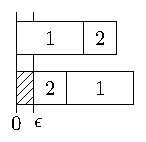
\includegraphics[width=0.2\textwidth]{figures/non-delay.pdf}
  \caption{Illustration of the two possible schedules for
    Example~\ref{eg:non-delay}. The first schedule is a non-delay schedule. The
    unforced idle time in the second schedule is shaded.}
  \label{fig:non-delay}
\end{figure}

% job families, precedence chains
Next, we consider \textit{precedence constraints} between jobs, which can be
used to fix a certain order among jobs. Suppose that job $j$ needs to be
processed before job $l$, denoted as $j \rightarrow{} l$, then we simply require
that $y_{l} \geq C_{j}$ in any feasible schedule. In particular, we may consider
\textit{chains} of precedence constraints. Let $F_{1}, \dots, F_{K}$ be a
partition of jobs into $K$ non-empty families. For each family $F_{k}$, we
require that their jobs $F_{k} = \{ J_{k1}, \dots, J_{k,n_{k}}\}$ are processed
in the order
\begin{align*}
J_{k1} \rightarrow{} J_{k2} \rightarrow{} \dots \rightarrow{} J_{k,n_{k}} .
\end{align*}
Therefore, $J_{km}$ denotes the $m$th job of family $k$.
Note that the order between jobs from different families is unspecified, which
means that the scheduler may decide to \textit{merge} these chains arbitrarily.

% setup (switch-over) times
When job $j$ is directly followed by job $l$, we might want to introduce some
\textit{sequence-dependent setup time} $s_{jl} \geq 0$, by requiring that
$y_{l} \geq C_{j} + s_{jl}$. For our purposes, we will only consider setup times
depending on the family to which jobs belong. For $k_{1} \neq k_{2}$ and any pair
of jobs $j_{1} \in F_{k_{1}}$, $j_{2} \in F_{k_{2}}$, either the constraint
\begin{align*}
C_{j_{1}} + s_{k_{1},k_{2}} \leq y_{j_{2}}
\end{align*}
is satisfied or
\begin{align*}
C_{j_{2}} + s_{k_{2},k_{1}} \leq y_{j_{1}}.
\end{align*}

\textit{\color{blue}Is this the right moment to discuss generalized precedence
  constraints? Maybe it is better to defer this to the discussion on augmenting
  the disjunctive graph.}

\subsection{Problem Formulation}

% translate into pure scheduling problem
Using the modeling elements introduced above, we now pose the traffic control
problem as a single machine scheduling problem. The intersection is represented
as the single machine. Let each of the $n$ vehicles be represented by some job
$j$ with release date $r_{j}$. The starting time $y_{j}$ models the planned
crossing time of vehicle $j$, which needs to be determined by the traffic
controller. We will now show how the two types of constraints are formulated.

% constraints
Let $n_{k}$ denote the total number of vehicles arriving to lane $k$. For each
lane, we define a family $F_{k}$ consisting of all vehicles that arrive to it.
We assume, without loss of generality, that the jobs are ordered according to
non-decreasing release dates. Therefore, the first type of
constraints~\eqref{eq:traffic-constr-1} for each lane is modeled by a chain
of precedence constraints on each family by assuming that
\begin{align*}
  r_{J_{kn}} < r_{J_{km}} \implies n < m ,
\end{align*}
for any pair of jobs $J_{kn}, J_{km} \in F_{k}$. \textit{\color{blue}This way of writing may seem confusing. Note that $J_{km}$ is really just a ``partial'' permutation, so maybe writing $J_{k}(n)$ is clearer.}

It is not difficult to see
that the second set of constraints~\eqref{eq:traffic-constr-2} for vehicles from
different lanes can be directly modeled using setup times $s_{k_{1},k_{2}}$. In
what follows, we will also refer to this setup time as \textit{switch-over}
time, because it is similar to the time between switching \textit{phases} in
convential traffic lights.

% objective
Because the release dates $r_{j}$ and processing time $p_{j}$ are assumed to be
known a priori, observe that minimizing the total delay ~\eqref{eq:total-delay}
experienced by all vehicles is equivalent to minimzing the total completion time,
so this is the objective that we will use from here one.

\begin{define}[Single Intersection Scheduling Problem]
  \label{def:single-problem}
  The single machine scheduling problem with release dates, job families with
  chain precedence constraints, family-dependent setup times and total
  completion time objective is called the {\normalfont single intersection
    scheduling problem}. In the three-field notation
  \cite{grahamOptimizationApproximationDeterministic1979}, we will denote it as
  $1 \, | \, r_{j}, \text{fmls}, \text{chains}, s_{gh} \, | \sum C_{j}$.
\end{define}

When vehicles turn at the intersection, the safe switch-over time between
vehicles depends on the involved lanes, because some turns take more time to
complete than others, see Figure~\textit{\color{blue}todo (see Limpens' Figure
  13)} for an illustration. For the moment, we will assume that vehicles cross
the intersection without turning, which allows us to make the following
assumption.

\begin{assump}
  \label{assump1}
  The processing times $p_{j} = p$ and setup times $s_{k_{1},k_{2}} = s$ are all
  identical, for $j \in \{1, \dots, n\}$ and any pair of lanes $k_{1}$ and
  $k_{2}$.
\end{assump}

The chain precedence constraints require a minimum of $p$ time units between the
crossing times of two jobs from the same lane. This give rise to an additional
assumption that can be made on the specification of the release dates.

\begin{assump}
  \label{assump2}
  For each job family $F_{k} = \{ J_{k1} , \dots, J_{k,n_{k}} \}$, the release
  dates satisfy $r_{J_{km}} = \max\{ r_{J_{km}}, r_{J_{k,m-1}} + p \}$, for all
  $m \in \{2, \dots, n_{k}\}$, without loss of generality.
\end{assump}

\textit{\color{blue}At this point, we should have defined the Single Intersection Scheduling Problem clearly and completely. If you don't agree, please indicate what is missing or unclear. Also note that giving a MILP formulation is not always the best way to state a problem in general, because different formulations, although mathematically equivalent, can have very different solving time complexity.}


\subsubsection{Mixed-Integer Linear Progam}
\label{sec:single-MILP}

A common method of solving combinatorial problems in general and scheduling
problems in particular is by formulating a Mixed-Integer Linear Program (MILP)
and solving it using branch-and-bound methods. Let $\mathcal{C}$ denote the set
of all single precedence constraints $j \rightarrow l$, collected from all
family chains. Furthermore, let
\begin{align}
  \mathcal{D} = \{ \{j,l\} : j \in F_{k_{1}}, l \in F_{k_{2}}, k_{1} \neq k_{2} \}
\end{align}
denote all pairs of jobs from distinct families, to which we will refer as
\textit{conflict pairs}. The problem from Definition~\ref{def:single-problem}
under Assumptions~\ref{assump1} and \ref{assump2} can be stated as
%
\begin{subequations}
\begin{align}
  \text{minimize } & \sum_{j=1}^{n} C_{j} & \\
  \text{s.t. } & r_{j} \leq y_{j} & \text{ for all } j=1, \dots, n, \\
              & C_{j} \leq y_{l} & \text{ for all } j \rightarrow l \in \mathcal{C}, \\
              & C_{j} + s \leq y_{l} \text{ or } C_{l} + s \leq y_{j} & \text{ for all } \{j,l\} \in \mathcal{D}. \label{eq:natural-disjunctions}
\end{align}
\end{subequations}

Observe that the above so-called \textit{natural formulation} is not yet a
proper MILP, because of disjunctive constraints~\eqref{eq:natural-disjunctions}.
One way to resolve this issue is to explicitly encode the ordering decisions.
For each $(j,l) \in \mathcal{D}$, we could introduce a binary decision variable
$o_{jl}$. A value of $o_{jl} = 0$ indicates that vehicle $j$ goes before vehicle
$l$ and a value of $o_{jl} = 1$ indicates that $l$ goes before $j$. However,
note that this introduces unnecessary redundancy into the formulation, because
$o_{jl} = 1 - o_{lj}$ always hold. Therefore, we only need one variable for each
(unordered) pair of vehicles, so we make an explicity selection by defining
\begin{align}
  \bar{\mathcal{D}} = \{ (j,l) : \{ j,l \} \in \mathcal{D}, j < l \}.
\end{align}
Let
$M > 0$ denote a sufficiently large constant (which may depend on the current
problem instance), then using the well-known \textit{big-M method}, we transform
the above natural formulation into
%
\begin{subequations}
\begin{align}
  \text{minimize } & \sum_{j=1}^{n} C_{j} & \\
  \text{s.t. } & r_{j} \leq y_{j} & \text{ for all } j=1, \dots, n, \\
              & C_{j} \leq y_{l} & \text{ for all } j \rightarrow l \in \mathcal{C}, \\
              & C_{j} + s \leq y_{l} + o_{jl}M  & \text{ for all } (j,l) \in \bar{\mathcal{D}}, \label{eq:disjunctive-constraints} \\
              & o_{jl} \in \{ 0, 1 \} & \text{ for all } (j,l) \in \bar{\mathcal{D}} ,
\end{align}
\end{subequations}
which is now a proper MILP.

\subsubsection{Complexity}
% complexity
The problem of minimizing the total completion time with release dates (written
as $1 \, | \, r_{j} \, | \sum C_{j}$ in the three-field notation
\cite{grahamOptimizationApproximationDeterministic1979}) has been long known to
be NP-hard \cite{lenstraComplexityMachineScheduling1977}, so there is no hope in
finding a polynomial algorithm for the current more general problem unless
$\mathcal{P} = \mathcal{NP}$. Therefore, we must resort to exhaustive
branch-and-bound methods or heuristics. However, note that this only holds for
the problem in its full generality. It might be worthwhile to further study the
parameterized complexity, i.e., the complexity of the problem as a function of
one or more of its parameters \cite{cyganParameterizedAlgorithms2015}.
Specifically, it would be interesting to verify the complexity in case of a
fixed number of lanes.


\newpage

\subsection{Problem structure}
Let us consider a couple of simple examples that might help discover some structure in the problem.

\begin{eg}
  Consider the situation with $J_{1} = \{ 1 \}, J_{2} = \{ 2 \}$. When both
  vehicles have the same release dates $r_{1} = r_{2} = r$, the order in which
  they cross the intersection does not influence the optimal total completion
  time of $\sum C_{j} = p + (p + S + p) = 3p + S$. Now, assume that vehicle 1
  has a earlier release date, then it is easily seen that an optimal schedule
  requires vehicle 1 to go first.
\end{eg}
%
\begin{eg}
  \label{example2}
  Consider the situation with $J_{1} = \{ 1 \}, J_{2} = \{ 2, 3 \}$. We are
  interested in how the release dates influence the order of the jobs in an
  optimal schedule. We assume that $r_{3} = r_{2} + p$. Suppose $r_{1} = r_{2}$,
  then we see that $2, 3, 1$ is optimal, which resembles some sort of ``longest
  chain first'' rule (\textit{\color{blue} relate this to Algorithm 3.1.4 of
    Pinedo}). Now assume that $r_{2} < r_{1} + p + s$, otherwise $1, 2, 3$ is
  simply optimal, because there is no \textit{conflict} between the two lanes
  (\textit{\color{blue}we will make this more precise later}). Furthermore, set
  $r_{1} = 0$, without loss of generality. We compare the sequence $1, 2, 3$
  with $2, 3, 1$. The first has optimal
  $\sum C_{j} = p + (p+s+p) + (p+s+p+p) = 6p + 2s$, while the second sequence
  has optimal
  $\sum C_{j} = (r_{2} + p) + (r_{2} + p + p) + (r_{2} + p + p + s + p) = 3 r_{2} + 6p + s$.
  Therefore, we conclude that the second sequence is optimal if and only if
  \begin{align*}
    r_{2} \leq s/3 ,
  \end{align*}
  which roughly means that the ``longest chain first'' rule becomes optimal
  whenever the release dates are ``close enough''.
\end{eg}
%
\begin{figure}
  \centering
  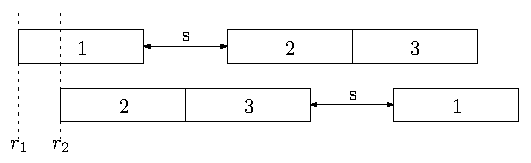
\includegraphics{figures/123.pdf}
  \caption{Illustration of the two possible sequences in Example~\ref{example2}.}
  \label{fig:example2}
\end{figure}
%
\begin{define}
  A sequence of consecutive jobs $n, n+1, \dots, n+m \in F_{l}$ from one lane is called a platoon if and only if $r_{i+1} = r_{i} + p$ for $n \leq i < n + m$.
\end{define}
%
\begin{eg}
  \label{example3}
  Suppose we have exactly two platoons of vehicles
  $J_{A} = \{ 1, \dots, n_{A}\}$, $J_{B} = \{ n_{A} + 1, \dots, n_{A} + n_{B}\}$,
  Assuming that
  $n_{A} < n_{B}$ and $r_{1} \leq r_{n_{A}+1}$, consider the ways the two platoons can merge by splitting A.
  Let $k$ denote the number of vehicles of platoon A that go after platoon B and
  let $\sum C_{j}(k)$ denote the resulting total completion time. We have
  \begin{align*}
    \sum C_{j}(0) = \sum_{i=1}^{n_{A}+n_{B}} ip + n_{B}s ,
  \end{align*}
  when A goes first and
  \begin{align*}
    \sum C_{j}(n_{A}+n_{B}) = \sum_{i=1}^{n_{A}+n_{B}} ip + n_{A}s ,
  \end{align*}
  when B goes first. For all the other cases, we have
  \begin{align*}
    \sum C_{j}(k) = \sum_{i=1}^{n_{A}+n_{B}} ip + n_{B}s + 2ks .
  \end{align*}
  From this analysis, we observe that it is not beneficial to split platoon A under the current assumptions. Moreover, we see that platoon B should go first, whenever
  \begin{align*}
    r_{n_{A} + 1} \leq (n_{B} - n_{A}) s / (n_{A} + n_{B}) .
  \end{align*}
\end{eg}
\begin{figure}
  \centering
  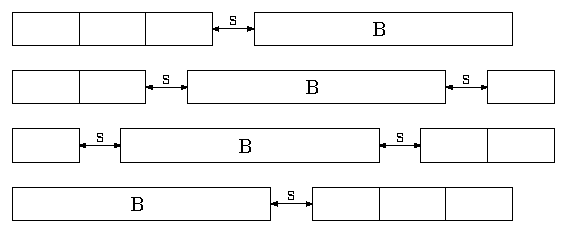
\includegraphics{figures/platoons.pdf}
  \caption{Illustration of splitting platoon A in Example~\ref{example3}.}
  \label{fig:example3}
\end{figure}

\begin{define}
  As the examples above show, the computation of the total completion time always includes a common term
  \begin{align*}
    \sum C_{j} = \sum_{i=1}^{n} ip + \dots ,
  \end{align*}
  which happens because of identical processing times
  (Assumption~\ref{assump1}). Therefore, we will from now on discard this term
  while comparing different schedules, by defining the {\normalfont total setup delay}
  \begin{align*}
    D = \sum C_{j} - \sum_{i=1}^{n} ip .
  \end{align*}
\end{define}

\subsubsection{Maximum vehicle delay}

Suppose we require that vehicles may not be delayed for longer than a fixed
maximum time $d_{\text{max}} \geq 0$. This means that the delay must satify
$y_{j} - r_{j} \leq d_{\text{max}}$, which implies that
$r_{j} \leq y_{j} \leq r_{j} + d_{\text{max}}$. A potential benefit of
introducing this maximum delay is that it could reduce the number of conflicts
between vehicles, which could make solving the MILP easier. However, it can also
cause the problem to become infeasible.

Consider a pair of conflicting vehicles $j, l$ and assume $r_{j} \leq r_{l}$,
without loss of generality. Observe that for
$d_{\text{max}} < r_{l} - r_{j} - p - s$, we do not need to worry about the
conflict anymore, because
$C_{j} + s = y_{j} + p + s \leq r_{j} + d_{\text{max}} + p + s < r_{l} \leq y_{l}$,
so the disjunctive constraint in \eqref{eq:disjunctive-constraints} can only
hold for $o_{jl} = 0$. In other words, the order of $j$ and $l$ is already
fixed, because the schedule is infeasible otherwise. Therefore, there is no real
conflict between vehicles $j$ and $l$, so $\{j, l\} \notin \mathcal{D}$.


\subsection{Single Platoon Positioning}

Focus on the problem with two lanes $F_{A}$ and $F_{B}$ where we assume that
there is only a single platoon arriving on lane $B$, i.e., the \textit{single
  platoon positioning problem}. In this case, the optimal schedule can be easily
computed by considering all positions. However, we use this simple case to
obtain some insight into when vehicles that are close act as if they were
platoons.

\begin{theorem}
  Under Assumption~\ref{assump1}, every vehicle scheduling problem must have an
  optimal schedule $y$ in which every platoon $p=(n, n+1, \dots, n+m)$ satisfies
  $y_{j+1} = y_{j} + p$ for all $n \leq j < n + m$.
  \textit{\color{blue}So this is the $x_i=0$ case.}
\end{theorem}
\begin{proof}
  Assume there exists an optimal schedule $y$ in which some platoon
  $P=(n, n+1, \dots, n+m)$ is \textit{split} in two parts, i.e, there exists
  some $j > 0$ such that $y_{n+j} > y_{n+j-1} + p$. Whenever the platoon is
  split in more parts, the following argument can be applied exhaustively.

  \textit{\color{blue}instead of considering parts P1 and P2, just show how a
    single vehicle can be scheduled earlier and argue that this argument may be
    applied exhaustively}

  Let $P_{1}$ and $P_{2}$ denote the separate parts of the original platoon. Let
  $B$ denote the set of vehicles that have
  $C_{n+j-1} + s \leq y_{l} \leq y_{n+j} - s$, i.e., those that are scheduled
  between the two parts of $P$. Similarly, let $A$ be the set of vehicles that
  have $y_{l} \geq C_{n+m} + s$, i.e., those that are scheduled after $P_{2}$.

  Let $x$ be the time between the end of $P_{1}$ and the start of the first job
  in $B$. The time between the last job of $B$ and the first job of $P_{2}$ must
  be $s$, otherwise the total completion time can be simply decreased by
  shifting $P_{2}$ earlier in time. Let $y$ be the time between the end of
  $P_{2}$ and the start of the first job in $A$.

  Now put $P_{2}$ right after the end of $P_{1}$, such that
  $y_{n+j} = y_{n+j-1} + p$ and consider the resulting change in total
  completion time.

  \textit{\color{blue}explain our method of idle time times number of jobs method}
\end{proof}

Assume that the first vehicle on the intersection arrives from lane $A$.
We provide a criterium for vehicles from $A$ to be candidates for going before the $B$-platoon, with length (number of vehicles) $n_{B}$.

\begin{proposition}
  Assume there is a vehicle $0 \in F_{A}$ starting at $y_{0} = 0$. Let $x_{i}$
  denote the finish-start delay between vehicle $i-1$ and $i$ when scheduled as
  early as possible, so let
  \begin{align*}
    x_{i} = r_{i} - (r_{i-1} + p) .
  \end{align*}
  If there exists a smallest integer $i'$ such that $x_{i'} \geq 2s + n_{B}p$,
  then any vehicle $i \geq i'$ needs to go after $B$ in any optimal schedule.
\end{proposition}

\noindent
\textit{\textit{\color{blue}illustrate the two job case with the ``decision'' diagram}}

\subsubsection{Insertion Heuristic}

We propose a heuristic that constructs a schedule for two lanes by considering
the vehicles in order of arrival and iteratively inserting each next vehicle in
the current partial schedule.

As in the single platoon scheduling problem, let $F_{A}$ and $F_{B}$ denote two
lanes, but now we allow lane $B$ to have arbitrary ariving vehicles. For the
first platoon of $B$, find the single platoon position among vehicles of $A$.
Then for every next platoon of $B$, solve the single platoon positioning
problem, while treating the position of the previously scheduled platoons fixed.


The following example shows that the resulting schedule may not be optimal,
because the position of earlier scheduled platoons restricts the possible
positions of later platoons.
\begin{eg}
  \textit{\color{blue}come up with example}
\end{eg}


\newpage

\section{Network of Intersections}

% structure (of the network)
We now leave the single intersection case and turn to vehicles traveling through
a network of intersections. The network is modeled as a weighted directed graph
$G=(V,E)$, with nodes and arcs representing intersections and roads,
respectively. Vehicles can travel along a series of arcs that are connected. Let
$d(x,y)$ be defined as the \textit{distance} between nodes $x$ and $y$. We
assume there are no nodes of degree two, since their two incident arcs $(x,y)$
and $(y,z)$ could be merged into one arc $(x,z)$ with
$d(x,z) = d(x,y) + d(y,z)$, without loss of expressiveness. Each node of degree
one is called an \textit{external node} and models the location where vehicles
enter (\textit{entrypoint}) or exit (\textit{exitpoint}) the network. A node of
degree at least three is called an \textit{internal node} and models an
intersection.

% behavior (traveling through the network)
Let the route of vehicle $j$ be denoted by $R_{j}$, which is encoded as a
sequence of nodes. Vehicle $j$ enters the network at some external node
$R_{j}(0)$ at time $r_{j}$ and then visits the $n_{j}$ nodes
$R_{j}(1), \dots, R_{j}(n_{j})$ until it reaches the exitpoint
$R_{j}(n_{j} + 1)$, where it leaves the network.
% define common path and merge point
Given two routes $R_{j}$ and $R_{l}$, we define a common path
$p=(i_{1},\dots,i_{L})$ as a substring of some length $L$ of both routes
(including external nodes). We refer to the first node $i_{1}$ of a common path
as a \textit{merge point}. The set of all common paths for vehicles $j$ and $l$
is denoted by $P_{jl}$. The set of all merge points for vehicles $j$ and $l$ is
denoted by $M_{jl}$. See Figure~\ref{fig:intersection-graph-example} for an
illustration of the above concepts.

\begin{figure}[t]
  \centering
  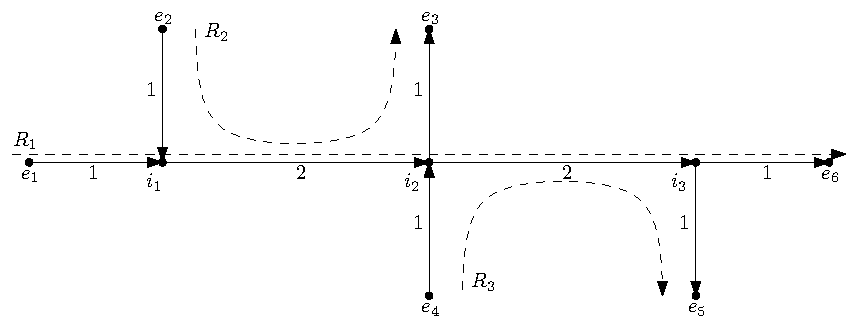
\includegraphics[width=1.0\textwidth]{figures/intersection-graph-example.pdf}
  \label{fig:intersection-graph-example}
  \caption{Example graph with three intersection $i_{1}, i_{2}, i_{3}$ and three
    vehicles, for which the routes are indicated by $R_{1}, R_{2}$ and $R_{3}$.
    The external nodes are labeled as $e_{1}, \dots, e_{6}$. The weight
    (distance) of each arc is indicated next to it. The common paths are
    $P_{12} = \{ (i_{1}, i_{2}) \}$, $P_{13} = \{ (i_{2}, i_{3}) \}$
    $P_{23} = \{ (i_{2}) \}$ and the corresponding merge points are
    $M_{12} = \{ i_{1} \}, M_{13} = \{ i_{2} \}, M_{23} = \{ i_{2} \}$.}
\end{figure}

% behavior on lanes
Vehicles are not able to overtake each other when traveling on the same arc. We
assume that arcs provide infinite \textit{buffers} for vehicles, meaning that
there is no limit on the number of vehicles that are traveling on the same arc
at the same time. However, we impose a minimum time required to travel along an
arc $(x,y)$. By assuming identical maximum speeds among vehicles, $d(x,y)$ can
be directly interpreted as this minimum travel time.

% constraints
Let $y_{ij}$ denote the time vehicle $j$ enters intersection $i$. Crossing the
intersection takes $p_{ij}$ time. Like in the single intersection case, we have
again two types of constraints. At most one vehicle can cross an intersection at
the same time (i), so when two consecutive vehicles crossing an intersection
originate from the same arc, they may pass immediately after each other. When a
vehicle $l$ that is about to cross next comes from a different arc than the
vehicle $j$ that last crossed the intersection, we require that there is at
least a \textit{switch-over time} $s_{jl}$ between the moment $j$ leaves and the
moment $l$ enters the intersection (ii).

% (scheduling) problem
Assuming that arrival times and routes of all vehicles are fixed and given, the
task of the traffic controller is to decide when individual vehicles should
cross intersections by determining $y$, while minimizing some measure of
optimality. This problem is similar to the classical job shop scheduling
setting, with intersections and vehicles now taking the roles of machines and
jobs, respectively. Therefore, we will first discuss this classical problem
before discussing how it should be adapted to fit the above setting.


\subsection{Job Shop Scheduling}

Assume there are $m$ machines and $n$ jobs that need to be processed on these
machines. A job $j$ consists of exactly $m$ operations, one for each of the
machines. We use the notation $(i,j)$ to denote the operation of job $j$ that
needs to be processed on machine $i$. The time required for processing operation
$(i,j)$ is denoted by $p_{ij}$. When a job only needs processing on a subset of
the machines, we can simply assume that $p_{ij} = 0$ for the machines that are
not involved. Like in the single machine case, we may define a release date
$r_{ij}$ for each operation, specifying the earliest time processing may start.
Let the set of all operations be denoted by $N$.

% machine order constraints
The order in which a job visits the machines is called the \textit{machine
  order} of this job. The machine order is given as part of the problem
specification and may be different for each job. An operation $(k,j)$ may only
start once its predecessor $(i,j)$ has completed processing, which means that
the precedence constraint $(i,j) \rightarrow (k,j)$ must be satisfied. In
general, machine order of a job is encoded as a chain of precedence constraints.
The set of all the pairs of operations to which such constraint applies is
denoted by $\mathcal{C}$.

% machine sequence constraints
Each machine $i$ can process at most one operation at the same time and, once
started, operations cannot be preempted. Therefore, the scheduler needs to order
the operations that need processing on $i$. We define the set of
\textit{conflict pairs}
\begin{align}
  \mathcal{D} = \{ \{(i,j), (i,l)\} : (i,j), (i,l) \in N \},
\end{align}
which generalizes the conflict pairs that we defined for the single intersection
in Section~\ref{sec:single-MILP}.

% problem formulation for makespan
Let $y_{ij}$ denote the time when operation $(i,j)$ starts processing, which
needs to be determined by the scheduler. A valid schedule is given by setting
values for $y_{ij}$ such that the above requirements are met. There are various
measures for how \textit{good} a given schedule is. For the purpose of the
discussion that follows, let us consider the well-known makespan objective
\begin{align}
\max_{(i,j) \in N} C_{ij},
\end{align}
where $C_{ij} = y_{ij} + p_{ij}$ is the completion time of
operation $(i,j)$. Minimizing the makespan often results in schedules that make
efficient use of the available machines and can now be formulated as
%
\begin{subequations}
  \label{eq:job-shop-natural}
\begin{align}
  \text{minimize } C_{\text{max}} \\
  \text{s.t. } C_{ij} &\leq y_{kj}  & \text{ for all } (i,j) \xrightarrow{} (k,j) \in \mathcal{C}, \\
  C_{il} &\leq  y_{ij} \text{ or } C_{ij} \leq y_{il}  & \text{ for all } \{(i,l), (i,j)\} \in \mathcal{D}, \label{eq:disjunctive-constraints} \\
  C_{ij} &\leq C_{\text{max}} & \text{ for all } (i,j) \in N, \\
  y_{ij} &\geq r_{ij} & \text{ for all } (i,j) \in N.
\end{align}
\end{subequations}
%
The first set of constraints enforces the machine order for each job. The second
set of constraints are called \textit{disjunctive}, because they model the
choice between jobs $j$ and $l$ to be scheduled first on machine $i$. The third
set of constraints are used to define the makespan and the last line enforces
the release dates.

% introduce s(i,j,l)
To support the following discussion, we introduce some additional notation.
Consider again the set of conflict pairs $\mathcal{D}$. For each conflict pair
$\{ (i,j), (i,l) \} \in \mathcal{D}$, the scheduler needs to make a binary
decision, i.e., it needs to decide whether jobs $j$ goes before job $l$ or vice
versa. Similarly to what we did in Section~\ref{sec:single-MILP}, we define the
auxilliary set
\begin{align}
  \bar{\mathcal{D}} = \{ (i,j,l) : \{ (i,j), (i,l) \} \in \mathcal{D}, j < l \} .
\end{align}
For each $(i,j,l) \in \bar{\mathcal{D}}$, we define the binary variable
$o(i,j,l)$ to encode the decision in the disjunctive constraints
\eqref{eq:disjunctive-constraints}. A value of zero corresponds to $j$ crossing
first and a value of one indicates that $l$ crosses first.

% travel time
Jobs may represent physical objects that need to be processed on machines.
Suppose we want to model the \textit{travel time} that is necessary to move the
job physically to the next machine. We can use so-called \textit{generalized
  precedence constraints} for this. We use the notation
\begin{align*}
  (i,j) \xrightarrow{d} (k,j)
\end{align*}
to indicate that operation $(i,j)$ is followed by operation $(k,j)$ and it takes
$d$ time to move the job from machine $i$ to $k$. This constraint can also be
formulated as
\begin{align}
  C_{ij} + d \leq y_{kj} .
\end{align}
Clearly, this generalizes the type of precedence constraints that we have been
using up till now (the original type is obtained by setting $d=0$).

\subsection{Problem Formulation}

The traffic control problem on a network of intersections can be modeled as a
job shop problem with generalized precedence constraints modeling the travel
times of vehicles and additional restrictions on the ordering of operations. As
in the single intersection case, intersections and vehicles are represented by
machines and jobs, respectively. Note that external nodes in $G$ are not
considered to be intersections.

% route and travel time (generalized prec. constraints)
For each job $j$, the machine order is given by the route $R_{j}$ of the
corresponding vehicle. The release date $r_{j}$ models the arrivals of vehicle
$j$ at its entrypoint $R_{j}(0)$. At internal nodes
$i \in \{R_{j}(1), \dots, R_{j}(n_{j})\}$, the starting time $y_{ij}$ models the
planned crossing time of vehicle $j$ at this intersection. The processing time
$p_{ij}$ models the amount of time necessary for safe crossing. Consider a pair
of consecutive nodes $(i,k)$ on the route $R_{j}$. The minimum time required to
travel is modeled by the generalized precedence constraint
\begin{align}
  (i,j) \xrightarrow{d(i,k)} (k,j) .
\end{align}
Again, we denote the set of all pairs of operations
$((R_{j}(n), j), (R_{j}(n+1), j))$ on consecutive pairs of nodes by
$\mathcal{C}$.


% restricting allowed orderings s
Now consider the decisions that need to be made regarding the ordering of
operations on the same machine, encoded by $o \in \{0,1\}^{\bar{\mathcal{D}}}$.
First of all, note that some binary vectors do not correspond to a feasible
schedule, because they encode a cycle of precedence constraints. By assuming
that vehicles cannot overtake each other while driving on the same lane, we are
further restricting the possible values of $o$. Consider a pair of vehicles
$j,l$. On each common path $(i_{1}, i_{2}, \dots, i_{L}) \in P_{jl}$, the order
cannot change, so we must have
\begin{align}
  o(i_{1},j,l) = o(i_{2},j,l) = \dots = o(i_{L},j,l).
\end{align}
% merge point if external node
A special case is when the merge point $i_{1}$ is an external node. In that
case, $i_{1}$ must be the entrypoint of both vehicles. That means that the order
on $p$ is determined by the order of arrival, which is determined by the release
dates. Therefore, we require $o(i_{1},j,l) = 1$ if $r_{j} > r_{l}$, and
$o(i_{1},j,l) = 0$ otherwise.
% summarize
Finally, let $\mathcal{O} \subset \{0,1\}^{\bar{\mathcal{D}}}$ denote the set of
all valid assignments to $o$.

% relation between o and y
We will now explain how the ordering decisions are related to the starting times $y$.
Note that $y_{ij}$ is only defined for internal nodes $i$.
% merge point is internal node
Consider an arbitrary triple $(i,j,l) \in \bar{\mathcal{D}}$. Suppose
$i \in M_{jl}$. In that case, the vehicles $j$ and $l$ approach $i$ from
different arcs, which means that switch-over time must be enforced, so we have
\begin{align}
  \begin{cases}
    (i,j) \xrightarrow{s} (i,l) & \text{ if } o(i,j,l) = 0 , \\
    (i,l) \xrightarrow{s} (i,j) & \text{ if } o(i,j,l) = 1 .
  \end{cases}
\end{align}
When $i$ is not a merge point, but it lies on some common path of $j$ and $l$,
then both vehicles are driving on the same lane, so we simply have
\begin{align}
  \begin{cases}
    (i,j) \xrightarrow{} (i,l) & \text{ if } o(i,j,l) = 0 , \\
    (i,l) \xrightarrow{} (i,j) & \text{ if } o(i,j,l) = 1 .
  \end{cases}
\end{align}
We merge these two cases by defining the switch-over time as
\begin{align}
  s(i,j,l) =
  \begin{cases}
    s & \text{ if } i \in M_{jl}, \\
    0 & \text{ otherwise },
  \end{cases}
\end{align}
%
which allows us to now compactly formulate the problem of minimizing total delay
in the network as
%
\begin{subequations}
\begin{align}
  \text{minimize } & \sum_{(i,j) \in N} C_{ij} \\
  \text{s.t. } & y_{ij} \geq r_{ij} & \text{ for all } (i,j) \in N, \\
  & (i,j) \xrightarrow{d(i,k)} (k,j) & \text{ for all } ((i,j), (k,j)) \in \mathcal{C} , \label{eq:travel-constraints} \\
  & (i,j) \xrightarrow{s(i,j,l)} (i,l) & \text{ if } o(i,j,l) = 0 , \text{ for } (i,j,l) \in \bar{\mathcal{D}}, \label{eq:common-path-constraints-1} \\
  & (i,l) \xrightarrow{s(i,j,l)} (i,j) & \text{ if } o(i,j,l) = 1 , \text{ for } (i,j,l) \in \bar{\mathcal{D}}, \label{eq:common-path-constraints-2} \\
  & o \in \mathcal{O}. \label{eq:common-path-order-constraints}
\end{align}
\end{subequations}

\begin{define}[Multi-Intersection Scheduling Problem]
  Given an intersection graph $G$, the job shop problem with release dates,
  graph travel time constraints \eqref{eq:travel-constraints}, machine-dependent
  setup times and no-overtaking constraint~\eqref{eq:common-path-constraints-1},
  \eqref{eq:common-path-constraints-2} and
  \eqref{eq:common-path-order-constraints} with total completion time objective
  is called the {\normalfont multi-intersection scheduling problem}. In the
  three-field notation, it could be denoted as \\
  $Jm \, | \, r_{j}, \text{graph}, s_{ijk}, \text{no-overtaking} \; | \sum C_{j}$.
\end{define}

In what follows, we will also make the following assumption.
\begin{assump}
The graph $G$ on which vehicles are travelling is acyclic and connected.
\end{assump}


\newpage

\subsection{Disjunctive graph}

% disjunctive graph
As an alternative to the natural formulation~\eqref{eq:job-shop-natural}, job
shop instance we can also be represented very clearly by their corresponding
\textit{disjunctive graph} (see Section 7.1 of
\cite{pinedoSchedulingTheoryAlgorithms2016} for a textbook introduction). Let
$(N, \mathcal{C}, \mathcal{D})$ be a directed graph with nodes $N$ corresponding
to operations and two types of arcs. The \textit{conjunctive} arcs $\mathcal{C}$
encode the given machine order for each job. If
$(i,j) \rightarrow (k, j) \in \mathcal{C}$ then job $j$ needs to be processed on
machine $i$ before it may be processed on machine $k$. The \textit{disjunctive}
arcs $\mathcal{D}$ are used to encode the decisions regarding the ordering of
jobs on a particular machine. For every conflict pair $\{(i,j), (i,l)\}$ of
different jobs $j$ and $l$ that need to be processed on the same machine $i$,
there is a pair of arcs in opposite directions between $(i,j)$ and $(i,l)$.
Therefore, each machine corresponds to a clique of double arcs between all the
operations that need to be performed on that machine.

For each machine $i$, the scheduler needs to order the operations that need processing on
$i$. This corresponds to choosing exactly one arc from every pair of opposite
disjunctive arcs. Let $\mathcal{D}' \subset \mathcal{D}$ be such a selection of
disjunctive arcs and let $G(\mathcal{D}')$ denote the resulting graph, to which
we will refer as a \textit{complete} disjunctive graph. It it not hard to see
that any feasible schedule corresponds to an acyclic complete disjunctive
graph.

Suppose we have $m=3$ machines and $n=3$ jobs. The first job has a machine order of 1,2,3 and the other two jobs have a machine order of 2,3,1.
Figure~\ref{fig:disjunctive-graph-example} shows the corresponding disjunctive graph for this instance.

\begin{figure}[t]
  \centering
  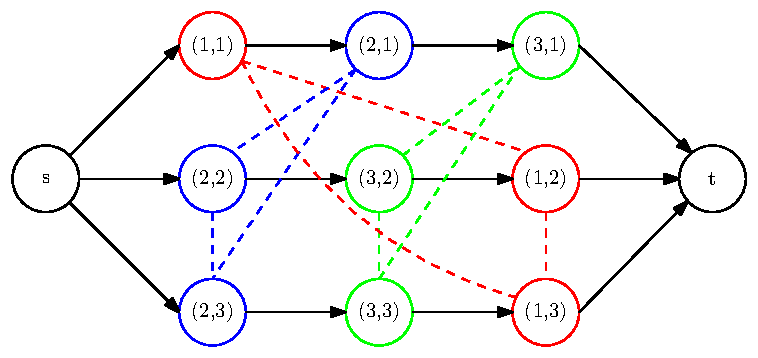
\includegraphics[width=0.5\textwidth]{figures/disjunctive-graph.pdf}
  \caption{Disjunctive graph corresponding to a job shop instance with three
    jobs and three machines. Operations that need to be scheduled on the same
    machine have been given the same color, emphasizing the cliques formed by
    their disjunctive arcs (drawn as dashed lines).}
  \label{fig:disjunctive-graph-example}
\end{figure}


\subsection{Schedule generation}
There are some classes of schedules that are relevant for job shop problems. The
following definitions are taken from the textbook by Pinedo
\cite{pinedoSchedulingTheoryAlgorithms2016}.

\begin{define}[Non-Delay Schedule]
A feasible schedule is called non-delay if no
machine is kept idle while an operation is waiting for processing.
\end{define}

\begin{define}[Active Schedule]
A feasible non-preemptive schedule is called active if
it is not possible to construct another schedule, through changes in the order
of processing on the machines, with at least one operation finishing earlier and
no operation finishing later.
\end{define}

\begin{define}[Semi-Active Schedule]
A feasible non-preemptive schedule is called
semi-active if no operation can be completed earlier without changing the order
of processing on any one of the machines.
\end{define}

It is clear that active schedules are necessarily semi-active, but the converse
does not always hold. Furthermore, when preemption is not allowed, non-delay
schedules are necessarily active. For some scheduling problems, it can be shown
that an optimal schedule exists that belongs to such classes.

\begin{eg}
  \label{eg:job-shop-non-delay}
  Consider two jobs on three machines with processing times
  $p_{\cdot 1} = \begin{pmatrix} 2 & 2 & 4 \end{pmatrix}^T$ and
  $p_{\cdot 2} = \begin{pmatrix} 1 & 2 & 1 \end{pmatrix}^T$. It is easily seen
  that the makespan is determined by
  $C_\text{max} = p_{11} + p_{21} + p_{31} = 8$ and an optimal schedule is given
  in Figure~\ref{fig:job-shop-delay}. This schedule is not non-delay, because
  machine 2 is kept idle from time 2 to 3, but operation $(2,2)$ could be
  scheduled here.
\end{eg}

\begin{figure}
  \centering
  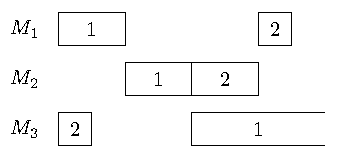
\includegraphics[width=0.5\textwidth]{figures/job-shop-delay.pdf}
  \caption{Optimal schedule for Example~\ref{eg:job-shop-non-delay}. The dashed
    lines indicate unit time steps. Machine 2 is kept idle, while operation
    $(2,2)$ could have already been scheduled at time 1.}
  \label{fig:job-shop-delay}
\end{figure}

For job shop problems, the optimal schedule is not necessarily non-delay, as the
example illustrates for the makespan objective. However, it can be
shown that $Jm || \gamma$ has an active optimal schedule, when $\gamma$ is a
regular objective, which means that it is a non-decreasing function of the
completion times $C_1, C_2, \dots, C_n$. The makespan and total completion time
are examples of regular objectives. Because of this result, branch-and-bound
methods have been proposed based on enumeration of all active schedules.

\vspace{0.5em}
\noindent
\textit{\color{blue}also active optimal schedule for $Jm | r_j | \gamma$?}

\begin{proposition}
  \label{prop:disjunctive-graph-semi-active}
  Every complete disjunctive graph corresponds to a unique semi-active schedule.
\end{proposition}
\begin{proof}
  Given some semi-active schedule, it is obvious that the corresponding
  disjunctive graph can be constructed by simply encoding the ordering of the
  operations in the schedule by the disjunctive arcs.

  We now argue that every complete disjunctive graph cannot correspond to more than
  one semi-active schedule.
  % introduce the longest path method lower bound on y = earliest starting time
  Recursively compute a lower bound on the starting time
  $LB(O_{jk}) = \max_{n \in O_{jk}^{-}} LB(n) + p_{jk}$ where $O_{jk}^{-}$ denotes
  the set of in-neighbors. In other words, $LB(O_{jk})$ is the longest path, when
  we associate weight $p_{jk}$ with every incoming arc of node $O_{jk}$ and add a
  dummy node $s$ with arcs to all first operations. Every feasible schedule $y$
  must satisfy $y_{jk} \geq LB(O_{jk})$. Hence, if any $y_{jk} > LB(O_{jk})$, then
  it is not semi-active.
\end{proof}

\begin{remark}
  After adding another dummy \textit{sink} node $t$ and adding arcs with weight
  zero from all the last operations to it, it is clear that
  $LB(t) = C_\text{max}$. This augmented disjunctive graph is shown in
  Figure~\ref{fig:augmented-graph} for the optimal schedule for
  Example~\ref{eg:job-shop-non-delay}.
\end{remark}

\begin{figure}
  \centering
  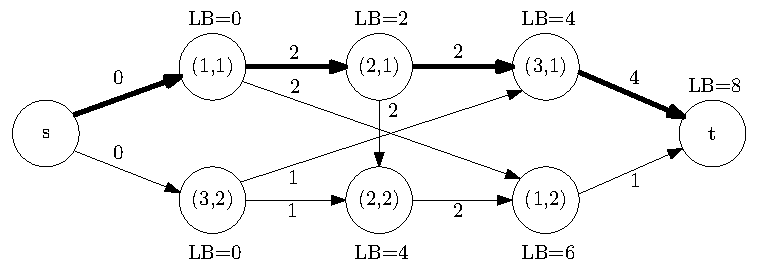
\includegraphics[width=0.9\textwidth]{figures/disjunctive-graph-source-sink.pdf}
  \caption{Disjunctive graph corresponding to
    Example~\ref{eg:job-shop-non-delay} augmented with source, sink and weights.
    The longest path determining the makespan $C_{\text{max}} = LB(t)$ is
    highlighted.}
  \label{fig:augmented-graph}
\end{figure}

\noindent
\textit{\color{blue}show how to adapt for total completion time (see Pinedo 7.3)}
\vspace{0.5em}

\noindent
\textit{\color{blue}Include here our solution of Exercise 7.11 from Pinedo,
i.e., a branching scheme for generating all schedules based on inserting
disjunctive arcs. From the resulting disjunctive graph, all semi-active
schedules follow by applying the machine makespan rule, introduced in the next
section.}


\subsection{Priority dispatching}

A \textit{priority dispatching rule} selects a job from a list of currently
available (unscheduled) jobs to be scheduled next. This produces a sequence
$\chi$ of jobs that are placed in a \textit{partial schedule}. Manually crafted
priority dispatching rules are mostly based on elementary features of the
current partial schedule. Well-known examples include the job with the
most/least work remaining (MWR/LWR) or the job with the shortest/longest
processing time (SPT/LPT).

Determining the dispatching sequence alone is not enough to obtain a schedule
$y$. The exact starting times are determined by a \textit{placement rule}. A
sensible placement rule would be to put the job in the earliest gap of idle time
where this job fits, i.e., where it can be placed without violating any
constraints. We call this the \textit{earliest gap} rule. Alternatively,
consider the straightforward placement rule that chooses the smallest starting
time $y_{ij}$ that satisfies $y_{ij} \geq y_{il} + p_{il}$ for all jobs $l$ that
have already been placed on machine $i$ in the current partial schedule and
$y_{ij} \geq y_{kj} + p_{kj}$, when $(k,j)$ is the preceding operation. We call
this the \textit{last position} rule, because the job is placed as the last job
on the machine.

% can dispatching rules generate all semi-active schedules?
We are now interested in whether scheduling with dispatching rules can generate
all necessary schedules. More precisely, we wonder whether all active schedules
can be generated from dispatching.

\begin{proposition}
  For every feasible semi-active schedule, there exists a sequence $\chi$ that
  generates it using the last position rule.
\end{proposition}
\begin{proof}
  Consider an arbitrary semi-active schedule $y$ and let $G$ be the
  corresponding complete disjunctive graph, which is unique by
  Proposition~\ref{prop:disjunctive-graph-semi-active} and has
  $y_{jk} = LB(O_{jk})$ for each node $O_{jk} \in N$. Because $G$ must be
  acyclic, there exists some topological ordering $\chi$ of the nodes.
  Therefore, dispatching in order of $\chi$ with the machine makespan rule will
  produce exactly the schedule with $y_{jk} = LB(O_{jk})$.
\end{proof}


\newpage

\section{Job Shop with Reinforcement Learning}

\subsection{Zhang et al.}

The authors of \cite{zhangLearningDispatchJob2020} use reinforcement learning to
solve the job shop problem with makespan objective $Jm || C_\text{max}$.
Specificaly, the method learns dispatching rules, so actions correspond to
selecting which (unfinished) job to schedule next. States are represented by a
disjunctive graph corresponding to the partial schedule. The policy is
parameterized by a graph neural network that reads the current disjunctive
graph. They use a dense reward based on the current lower bound of the makespan.



The state transition example shown in Figure~2 of
\cite{zhangLearningDispatchJob2020} suggests yet another placement rule, because
operation $O_{32}$ is placed before $O_{22}$, but it does not fit the gap.
Consequently, operation $O_{22}$ has to be delayed by three time steps.

\textit{\color{blue}Formalize the placement rule that Zhang et al. use and argue
that this does not guarantee that all active schedules can be generated in this
way.}



\subsection{Structure in Network Schedules}

Before we start experimenting with the above problem (see if the MIP method
scales and later trying to learn policies with (MA)RL), we first should try to
find some common structural patterns in solutions or even some simple general
scheduling rules.

\begin{itemize}
  \item Study simple situations with the total completion time objective ($\sum C_{j}$), in which some kind of LPT rule holds. (\textit{\color{blue} explain why LPT-like schedules arise})
  \item Study tandem networks where the $\sum C_{j}$ objective causes platoon splitting due to some kind of ``propagation of delay costs''. (\textit{\color{blue} insert the example that I have})
  \item Can we study this ``delay cost propagation'' using some kind of dependency graph, e.g., by recording that delaying job A would require us to also delay job B, which would also require to delay C, etc.?
\end{itemize}

\subsection{Platoon Splitting}

In the single intersection case, platoon splitting is never necessary. So in
this context, platoon splitting can only become necessary from using a different
performance metric, e.g., one that takes into account fairness. Once we start
looking at the network-level interactions, however, we can show that platoon
splitting is sometimes necessary to obtain an optimal schedule. The main idea is
that delaying a job $j$ might require to also delay further downstream jobs.
Therefore, it might be cheaper overall to not delay $j$, but interrupt some
already running job $l$ instead.


\section{Discussion}

We assumed that it is always possible to compute a speed profile, given a
feasible schedule $y$ for the scheduling problem. However, I think that certain
parameters like maximum acceleration and breaking influence the processing time
$p$ and the switch-over time $s$ that are necessary for this assumption to hold.

\vspace{0.5em}
\noindent
\textit{\color{blue}discuss multiple lanes, opposing lanes on the same arc and consider multiple phases at intersections}


\bibliography{references}
\bibliographystyle{ieeetr}

\end{document}
